\chapter{Regulator rozmyty}

W tej sekcji przedstawione zostaną wyniki symulacji działania przyjętego układu z regulatorem rozmytym Mamdaniego. Cały proces projektowania struktury regulatora został przeprowadzony w toolbox-ie \textit{Fuzzy} środowiska MATLAB. Głównym celem przeprowadzonych badań było zapoznanie się z zasadą działania regulatora rozmytego i  jak najlepsze odwzorowanie działania oryginalnego regulatora PD. \\
Zdecydowano, że sygnałami wejściowymi, na których bazował regulator będą uchyb i pochodna uchybu regulacji. Na bazie przebiegów wcześniej wspomnianych sygnałów została zaprojektowana baza reguł. Ze względu na różną dynamikę układu, zależną od wypełnienia szklanki, wprowadzono różne reguły dla sterowania. Wszystkie reguły w zależności od wartość uchybu regulacji i jego pochodnej podane są w tabeli \ref{fuzzy_table}. Symbole $P$ i $ P_p$ oznaczają odpowiednio regułę "dodatnią" dla pełnej i pustej szklanki.\\
W ramach przeprowadzonych badań symulacyjnych porównano działania regulatora na bazie wcześniej przyjętych wska\'zników jakości dla różnych postaci funkcji przynależności.

\begin{table}[h]
	\caption{Tabla reguł regulatora fuzzy. $N$ - wart. ujemna, $Z$ - wart. zerowa, $P$ - wart. dodatnia, $P_p$ - wart dodatnia dla pustej szklanki}
	\label{fuzzy_table} 
	\centering
	
	\begin{tabular}{|c|M{2.5cm}|M{2.5cm}|M{2.5cm}|}
		\hline
		$e / \dfrac{de(t)}{dt}$ &$N$&$Z$&$P$\\
		\hline
		$N$ &$Z$& $N$ & $N$\\
		\hline
		$Z$ &$N$& $Z$ & $P$\\
		\hline
		$P$ &$P_p$&  $P_p$ & $Z$\\
		\hline
		
	\end{tabular}
\end{table}

\section{Pierwszy zestaw funkcji przynależności}


\begin{figure}[h!]
	\centering
	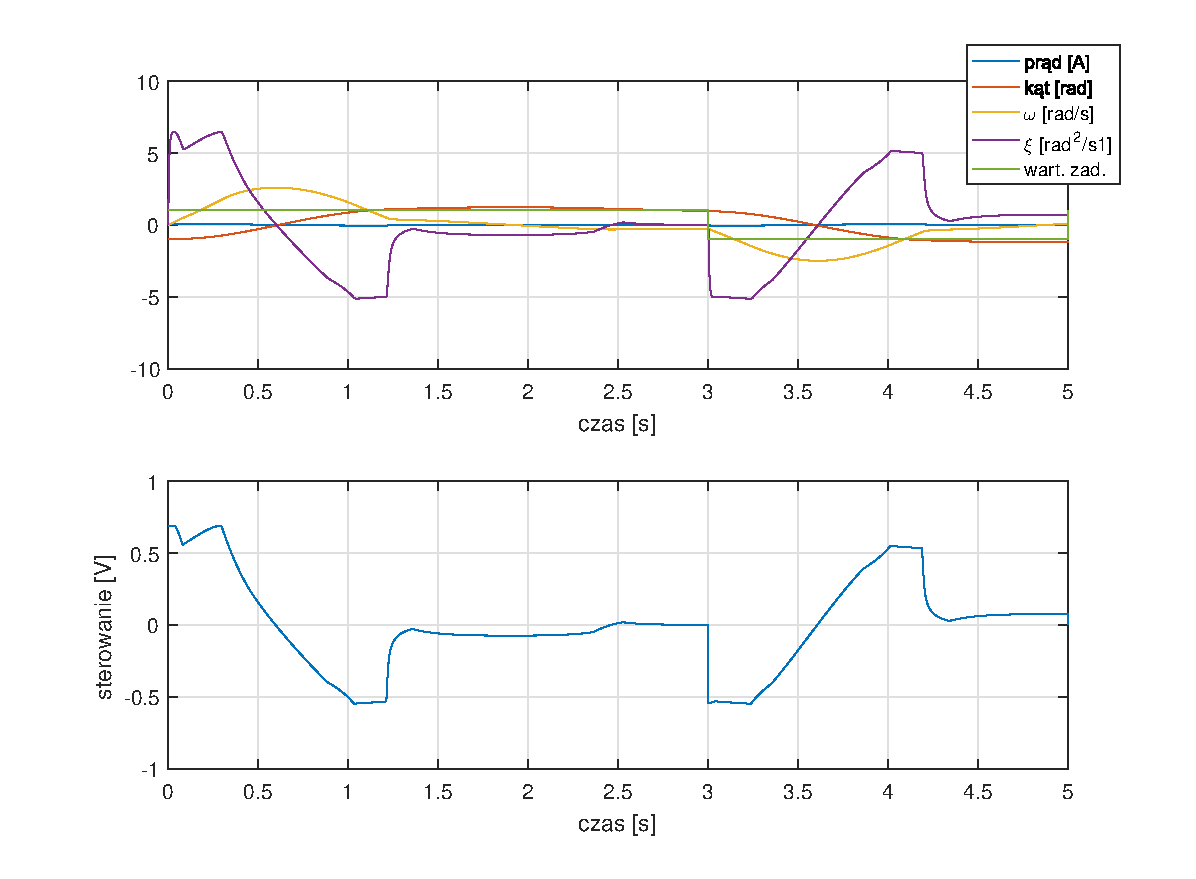
\includegraphics[scale = 0.8]{fig/fuzzy_odp.eps}
	\caption		
	{Odpowied\'z obiektu dla regulatora rozmytego.}
	\label{fuzzyOdp}
\end{figure}

 \begin{figure}[h!]
	\noindent\makebox[\textwidth]{
		\centering
		\subfloat[][Reguły dla uchybu regulacji.]{
			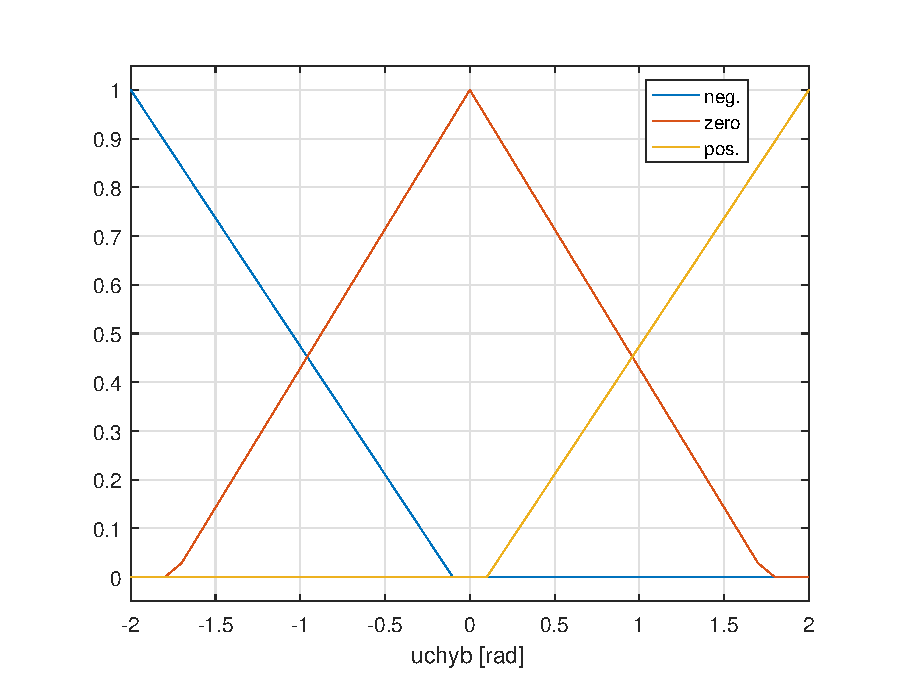
\includegraphics[scale=0.65]{fig/e_rules.eps}
			\label{e_rules1}
		}
		\hfill
		%\begin{figure}[h!]
		%	\centering
		\subfloat[][Reguły dla pochodnej uchybu.]{
			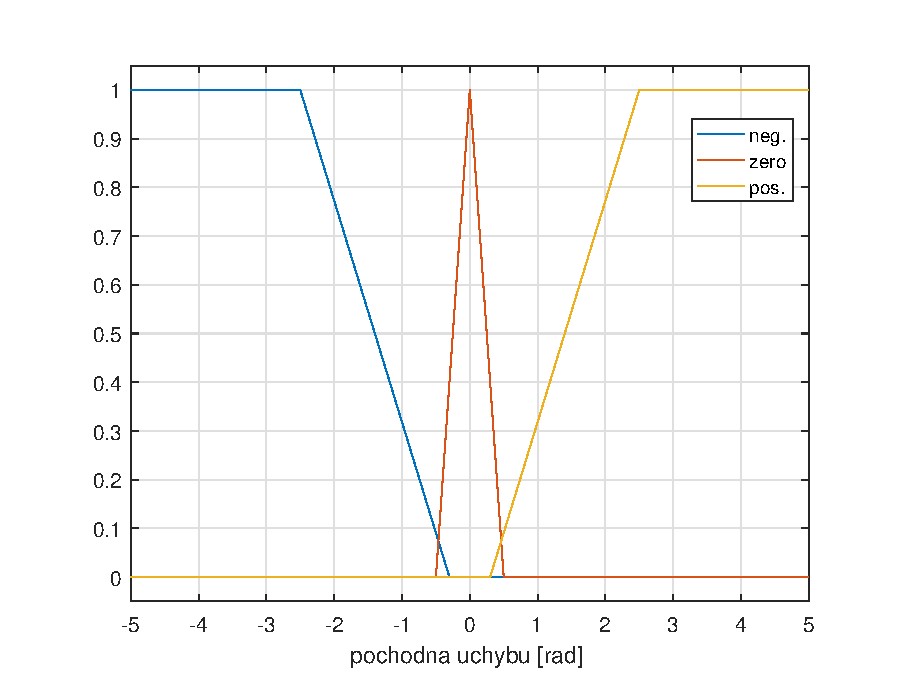
\includegraphics[scale=0.65]{fig/de_rules.eps}
			\label{de_rules1}
		}
		
		%{a) Porównanie wyjścia obiektu i estymaty. b) Porównanie błędów wyjścia i estymaty.}
	}
	\caption{Reguły dla pierwszego zestawu funkcji przynależności.}		
\end{figure}

\begin{figure}[h!]
	\centering
	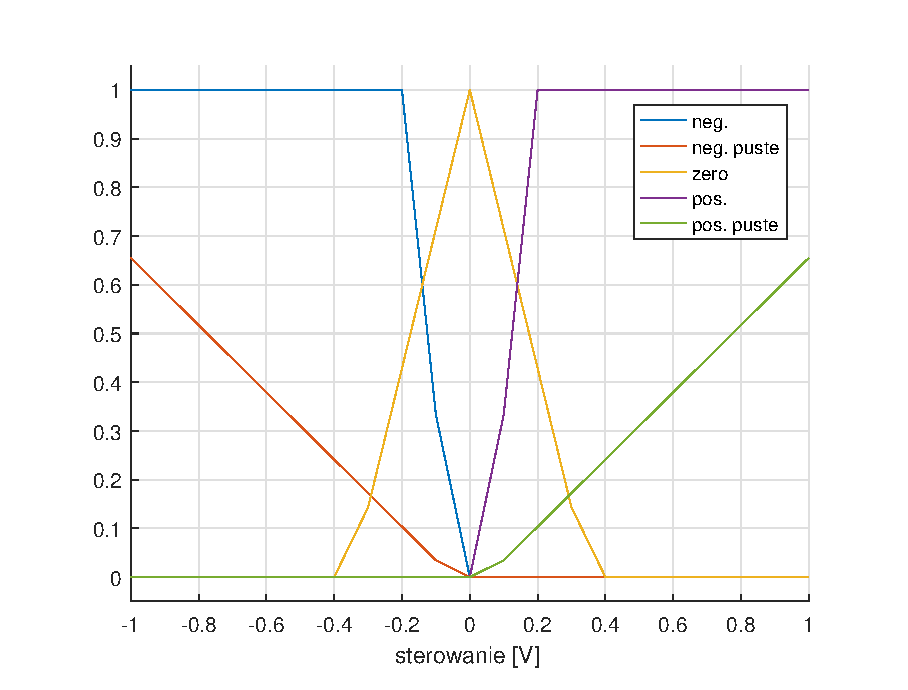
\includegraphics[scale = 0.65]{fig/u_rules.eps}
	\caption		
	{Reguły dla sterowania -  I zestaw funkcji przynależności.}
	\label{u_rules1}
\end{figure}

\FloatBarrier
\section{Drugi zestaw funkcji przynależności}
\label{mamdani2}
Na rysunku \ref{set2_surface} zaprezentowano płaszczyznę wyznaczoną przez przyjęte reguły.
\begin{figure}[h!]
	\centering
	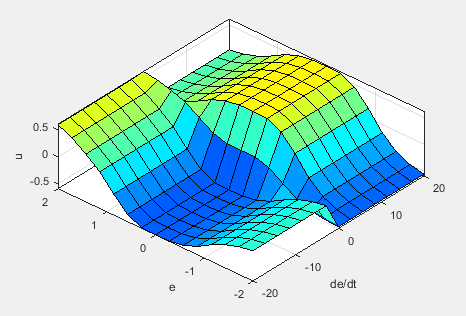
\includegraphics[scale = 0.8]{fig/fuzzySurface.PNG}
	\caption		
	{Płaszczyzna sterowań wyznaczona przez reguły zestawu nr II.}
	\label{set2_surface}
\end{figure}

\begin{figure}[h!]
	\centering
	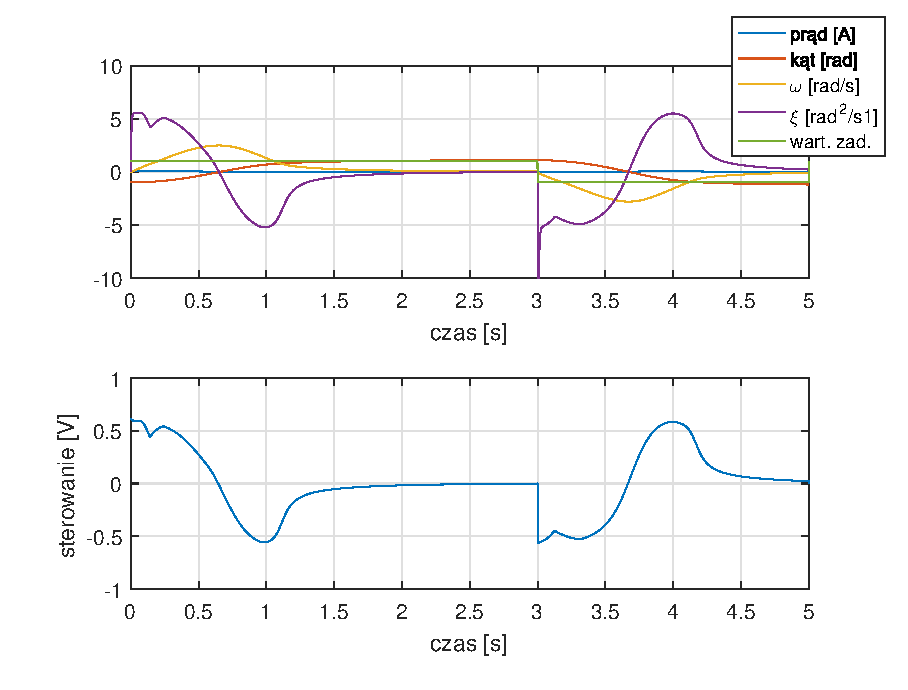
\includegraphics[scale = 1]{fig/fuzzy_odp2.eps}
	\caption		
	{Odpowied\'z obiektu dla regulatora rozmytego, II zestaw funkcji przynależności.}
	\label{fuzzyOdp2}
\end{figure}

 \begin{figure}[h!]
	\noindent\makebox[\textwidth]{
		\centering
		\subfloat[][Reguły dla uchybu regulacji.]{
			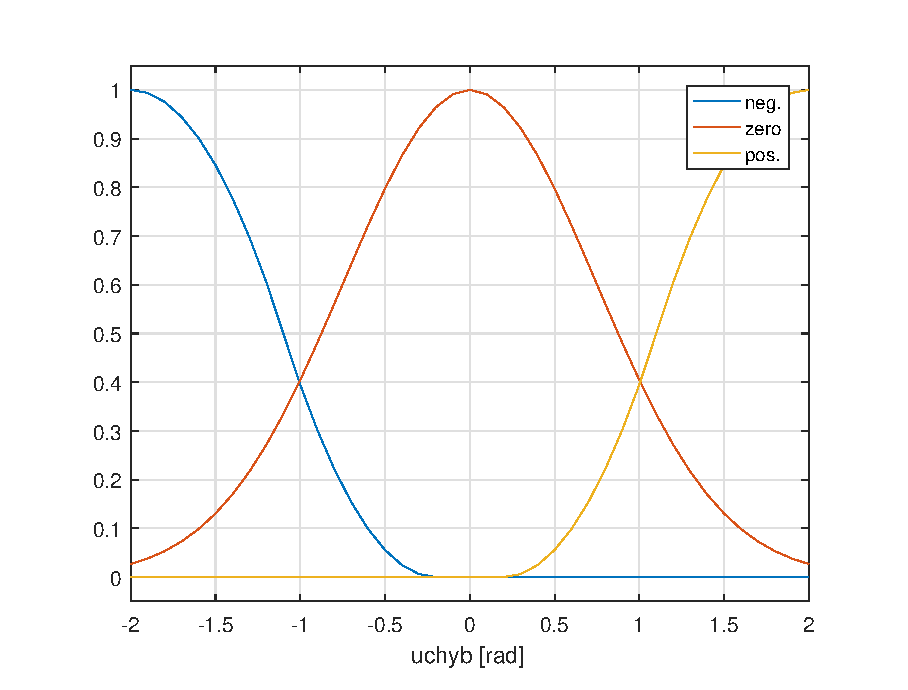
\includegraphics[scale=0.65]{fig/e_rules2.eps}
			\label{e_rules2}
		}
		\hfill
		%\begin{figure}[h!]
		%	\centering
		\subfloat[][Reguły dla pochodnej uchybu.]{
			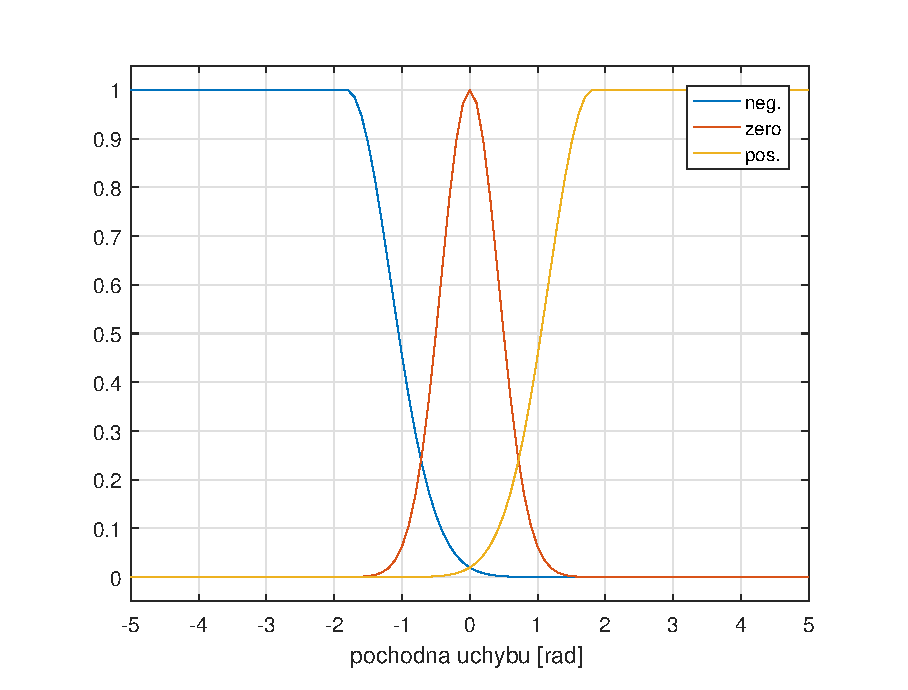
\includegraphics[scale=0.65]{fig/de_rules2.eps}
			\label{de_rules2}
		}
		
		%{a) Porównanie wyjścia obiektu i estymaty. b) Porównanie błędów wyjścia i estymaty.}
	}
	\caption{Reguły dla drugiego zestawu funkcji przynależności.}		
\end{figure}

\begin{figure}[h!]
	\centering
	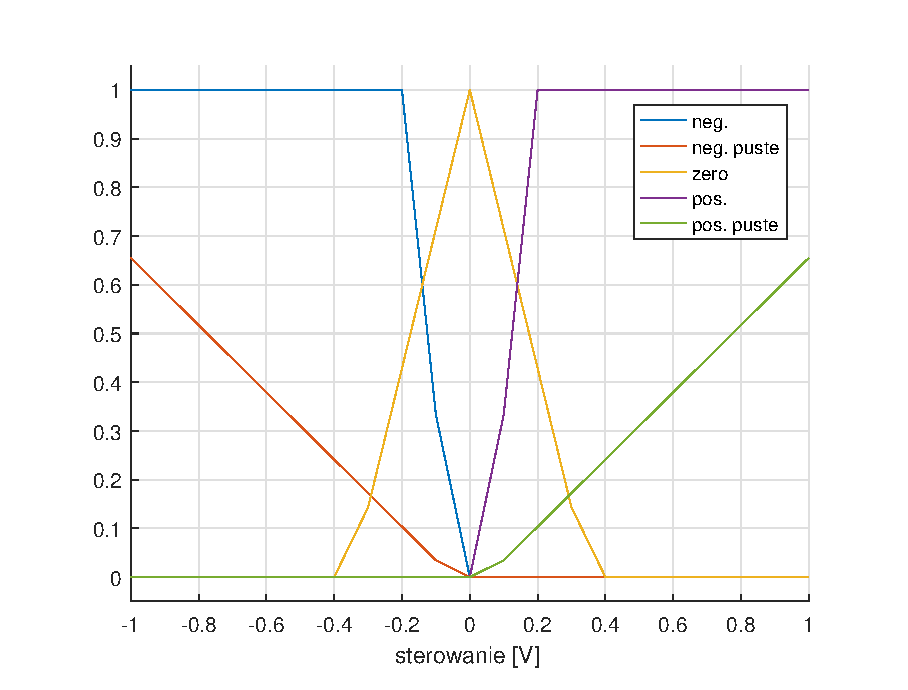
\includegraphics[scale = 0.65]{fig/u_rules.eps}
	\caption		
	{Reguły dla sterowania -  II zestaw funkcji przynależności.}
	\label{u_rules2}
\end{figure}
\FloatBarrier

\section{Porównanie}

Na rysunku \ref{fuzzy_por} przedstawiono porównanie przebiegów odpowiedzi obiektu dla każdego z rozpatrywanych zestawów reguł. W tabeli \ref{fuzzy_wsk} zapisano wartości wska\'zników jakości dla obu rozpatrywanych przypadków.
\begin{figure}[h!]
	\centering
	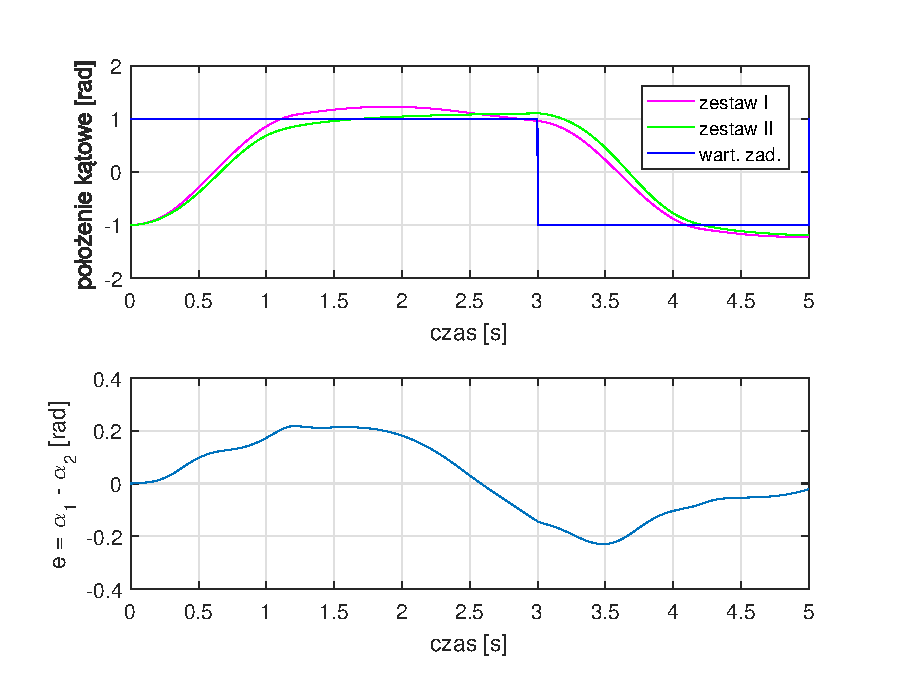
\includegraphics[scale = 1]{fig/por_fuzzy_sets.eps}
	\caption		
	{Porównanie działania regulatora dla oby zestawów reguł.}
	\label{fuzzy_por}
\end{figure}

\begin{table}[h]
	\caption{Wska\'zniki jakości dla regulatora PD - fuzzy.}
	\label{fuzzy_wsk}
	\centering
	
	\begin{tabular}{|c|M{2.5cm}|M{2.5cm}|M{2.5cm}|}
		\hline
		Funkcje przynależności &$J_1$&$J_2$&$J_3$\\
		\hline
		I zestaw &3.624&  1.96 &  5.583\\
		\hline
		II zestaw &4.201&  1.667 &  5.868\\
		\hline
				
	\end{tabular}
\end{table}
\newpage
\section{Regulator Takagi - Sageno}
Główną różnicą pomiędzy regulatorem rozmytym typu Takagi-Sageno (1985 r.), a strukturą regulatora zaproponowaną przez Mamdaniego jest liniowa funkcja wyjścia.  

\subsection{Manualny dobór struktury regulatora}
W rozpatrywanym przypadku reguły przynależności do zbiorów rozmytych dla sygnału wejściowego są identyczne jak te opisane w podrozdziale \ref{mamdani2}. Wielkościami poszukiwanymi w tym przypadku były wartości funkcji wyjściowej dla każdego z rozpatrywanych przypadków. Przyjęto, że będzie ona przyjmować wartości ze zbioru ${-1, 0, 1}$. W tabeli \ref{sagenoRulesTab} zamieszczone są wszystkie reguły zaprojektowanego regulatora.
\begin{table}[h!]
	\caption{Tabelka reguł regulatora typu Takagi-Sageno.}
	\label{sagenoRulesTab}
	\centering
	
	\begin{tabular}{|c|M{2.5cm}|M{2.5cm}|M{2.5cm}|}
		\hline
		$e / \dfrac{de(t)}{dt}$ &$N$&$Z$&$P$\\
		\hline
		$N$ &$0$& $-1$ & $-1$\\
		\hline
		$Z$ &$-1$& $0$ & $1$\\
		\hline
		$P$ &$1$&  $1$ & $0$\\
		\hline
		
	\end{tabular}
\end{table}
\FloatBarrier
%
Jak można zauważyć, tabela \ref{sagenoRulesTab} jest analogiczna do tabeli \ref{fuzzy_table} z tą różnicą, że nieliniowe funkcje przynależności zastąpiono liczbami.\\
Na rysunku \ref{fuzzy_sageno_sufraceMan} zaprezentowano powierzchnię sterowania dla tak dobranej struktury regulatora, a na rysunku \ref{fuzzy_sageno_man} odpowied\'z układu.\\
\begin{figure}[h!]
	\centering
	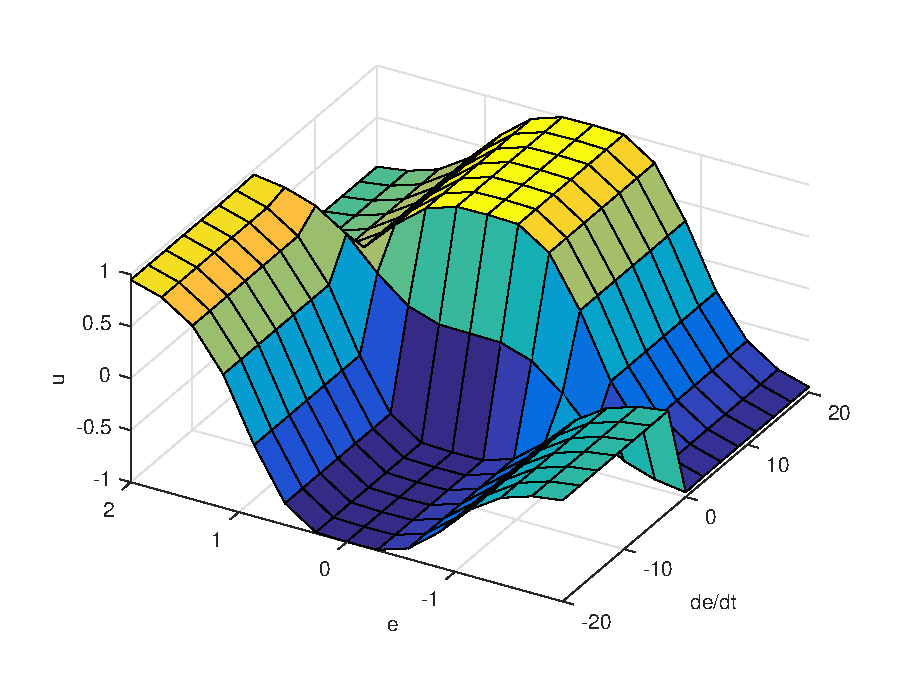
\includegraphics[scale = 0.7]{fig/sagenoManSurface.eps}
	\caption		
	{Powierzchnia sterowania dla regulatora rozmytego typu Takagi-Sageno.}
	\label{fuzzy_sageno_sufraceMan}
\end{figure}

\begin{figure}[h!]
	\centering
	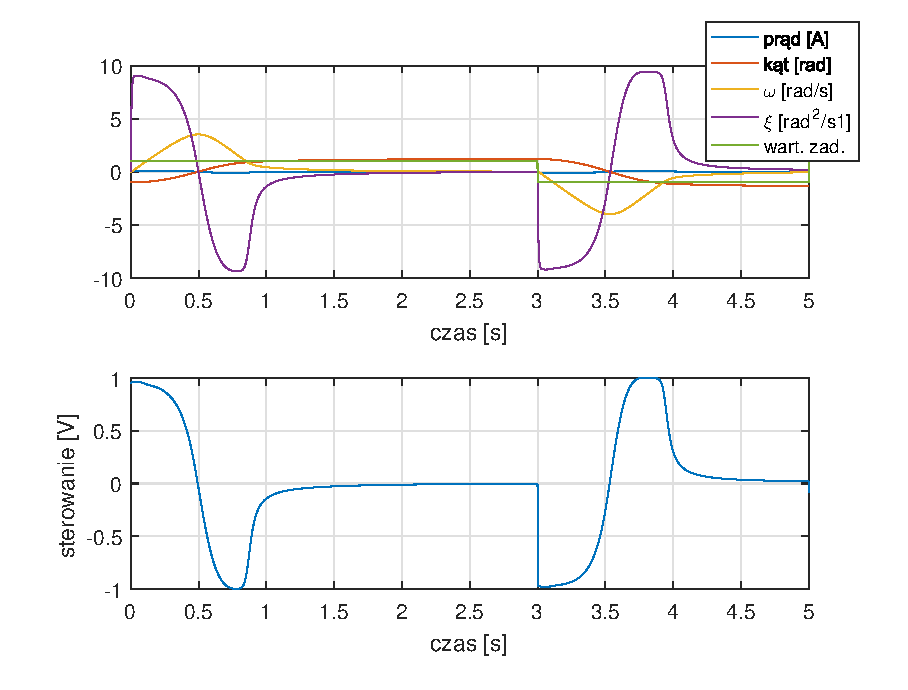
\includegraphics[scale = 0.8]{fig/fuzzy_sagenoMan_odp.eps}
	\caption		
	{Odpowied\'z obiektu dla regulatora rozmytego typu Takagi-Sageno.}
	\label{fuzzy_sageno_man}
\end{figure}
\FloatBarrier
\newpage

\subsection{Optymalizacja struktury regulatora}
W kolejnym kroku wykorzystano funkcje środowiska Matlab \textit{genfis1} i \textit{anfis} do wyznaczenia struktury regulatora. W procesie konfiguracji ustawiono gaussowskie funkcje przynależności zarówno dla uchybu regulacji jak i dla jego pochodnej. Na rysunkach \ref{fuzzy_sageno_sufrace} - \ref{fuzzy_sageno_e_rulles} zaprezentowano płaszczyznę sterowania oraz funkcje przynależności zwrócone przez wcześniej wymienione funkcje.
\begin{figure}[h!]
	\centering
	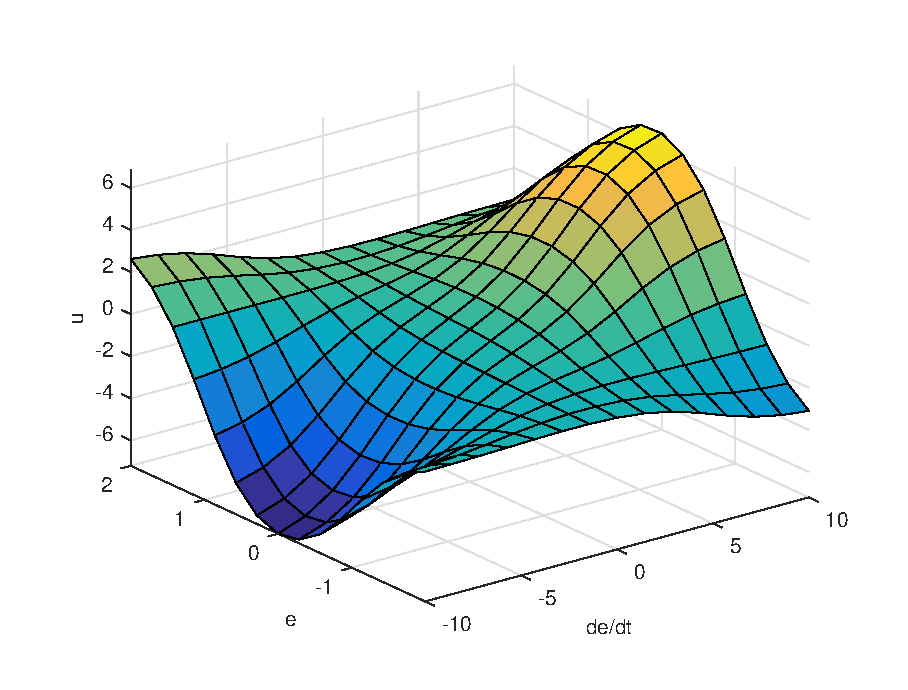
\includegraphics[scale = 0.8]{fig/sagenoOptSurface.eps}
	\caption		
	{Powierzchnia sterowania dla regulatora rozmytego typu Takagi-Sageno po optymalizacji.}
	\label{fuzzy_sageno_sufrace}
\end{figure}

 \begin{figure}[h!]
 	\noindent\makebox[\textwidth]{
	\centering
	\subfloat[][Reguły dla uchybu regulacji.]{
		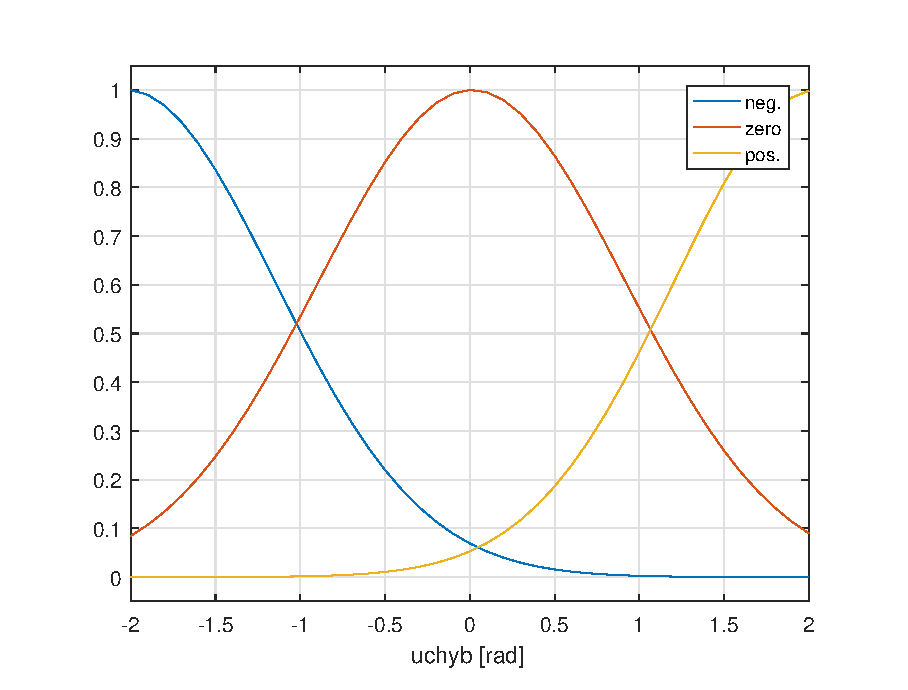
\includegraphics[scale=0.65]{fig/e_rules_sageno.eps}
		\label{fuzzy_sageno_e_rulles}
	}
	\hfill
	%\begin{figure}[h!]
	%	\centering
	\subfloat[][Reguły dla pochodnej uchybu.]{
		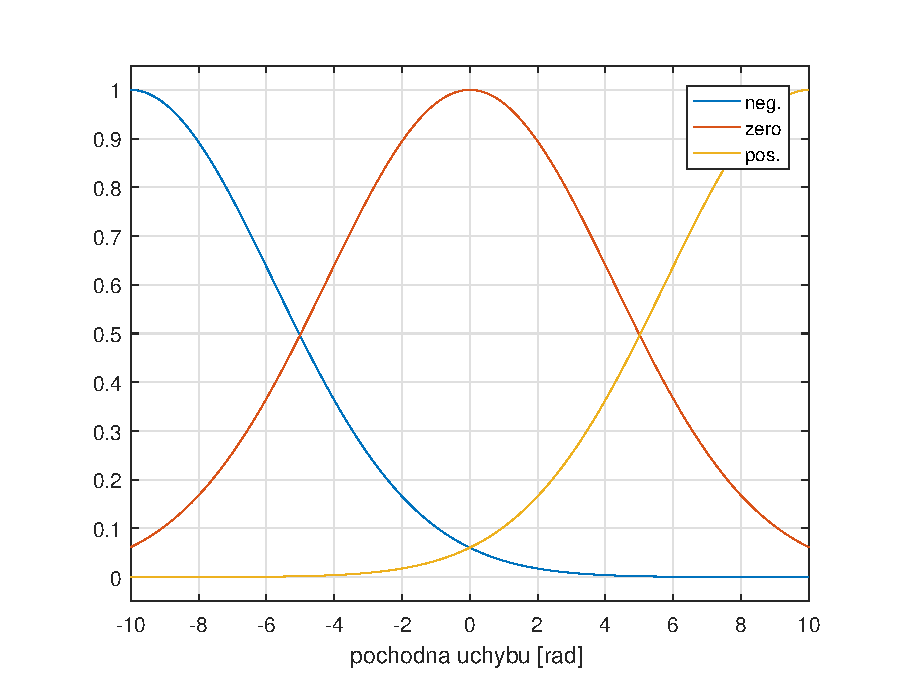
\includegraphics[scale=0.65]{fig/de_rules_sageno.eps}
		\label{fuzzy_sageno_de_rulles}
	}

	%{a) Porównanie wyjścia obiektu i estymaty. b) Porównanie błędów wyjścia i estymaty.}
	}
\caption{Reguły dla regulatora T-S po optymalizacji.}		
\end{figure}

\FloatBarrier
Rysunek \ref{fuzzy_sageno_odp} przedstawia przebiegi wszystkich zmiennych stanu rozważanego układu.
\begin{figure}[h!]
	\centering
	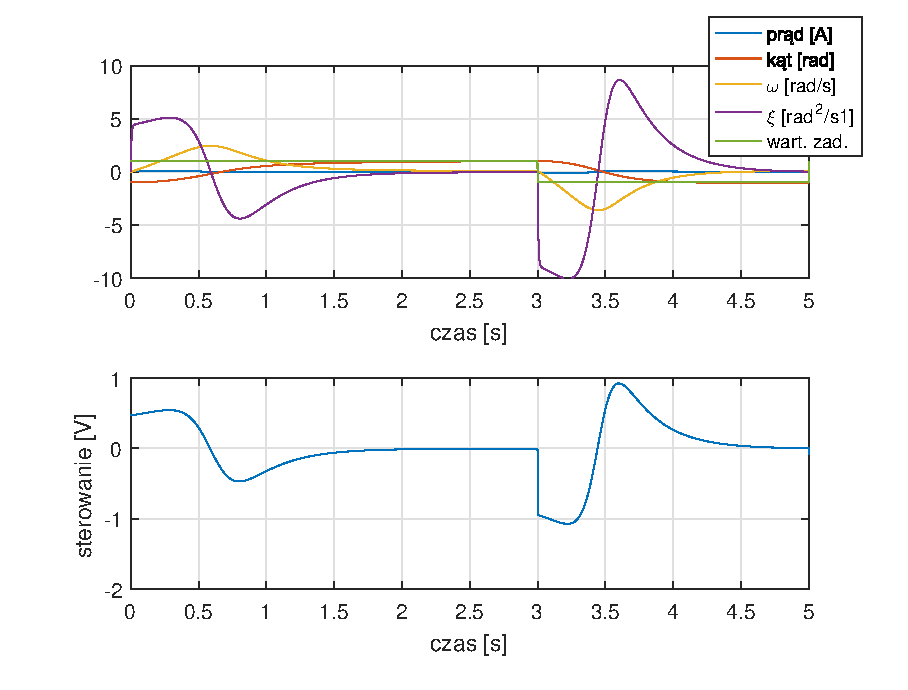
\includegraphics[scale = 1]{fig/fuzzy_sagenoOpt_odp.eps}
	\caption		
	{Odpowied\'z obiektu dla regulatora rozmytego typu Takagi-Sageno po optymalizacji.}
	\label{fuzzy_sageno_odp}
\end{figure}

\subsection{Porównanie}
\begin{figure}[h!]
	\centering
	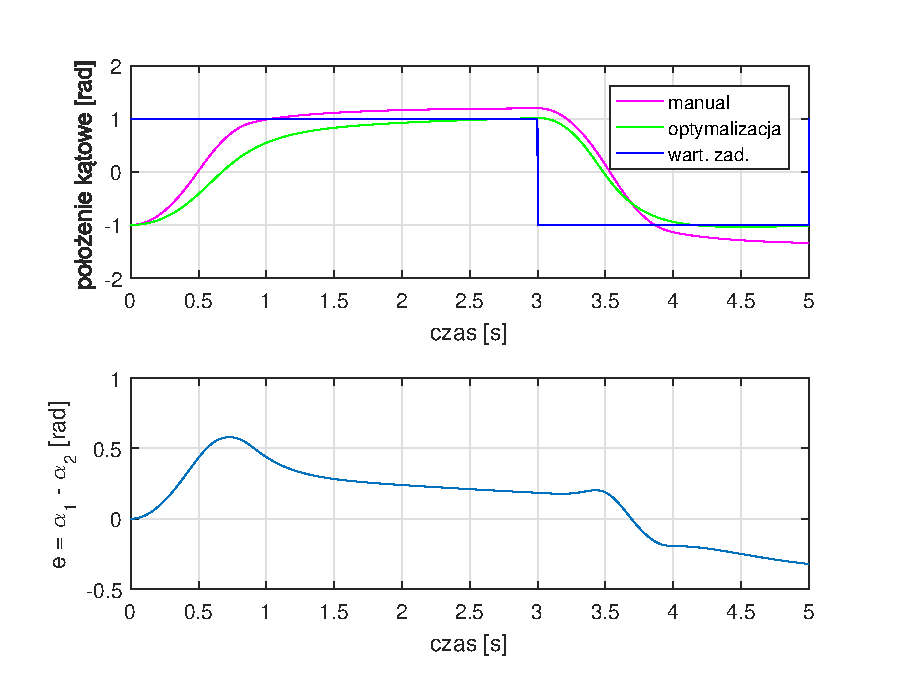
\includegraphics[scale = 0.8]{fig/por_fuzzy_sageno.eps}
	\caption		
	{Porównanie działania regulatora przed i po optymalizacji.}
	\label{fuzzy_sageno_por}
\end{figure}

\begin{table}[h]
	\caption{Porównanie wska\'zników jakości dla regulatora rozmytego typu Takagi-Sageno.}
	\label{fuzzy_sageno_wsk}
	\centering
	
	\begin{tabular}{|c|M{2.5cm}|M{2.5cm}|M{2.5cm}|}
		\hline
		Sposób projektowania &$J_1$&$J_2$&$J_3$\\
		\hline
		manualny &3.497&  2.639 &  6.136\\
		\hline
		optymalizacja &3.642&  0.8707 &  4.513\\
		\hline		
	\end{tabular}
\end{table}